\section{Results and evaluation}
In this section we will discuss the performance of both our simple and complex models, and discuss how these stack up
against eachother. We will discuss the accuracy and performance on both the FakeNewsCorpus dataset and the LIAR
dataset. And we will end of this evaluation by discussing the challenges in general fake news classifiers, and the
ethical and practical challenges such a model encounters.

\subsection{Relative performance on FakeNewsCorpus}
Let's begin by looking at our models performance on the FakeNewsCorpus dataset. As we see from table \ref{tab:fakenewsperformance},
all of our models performed admirably when being run against the test set, with our more complex models pulling ahead
comfortably.

\begin{table}[htpb]
  \centering
  \caption{Model performance on FakeNewsCorpus dataset}
  \label{tab:fakenewsperformance}

  \begin{tabular}{c|cccc}
    Model & Logistic Regression & Large DNN & Small DNN & XGBoost \\ \hline
    Precision (Reliable / Unreliable) & 0.95 / 0.98 & 0.83 / 0.94 & 0.92 / 0.98 & 0.87 / 0.95 \\ \hline
    Recall (Reliable / Unreliable) & 0.95 / 0.98 & 0.87 / 0.92 & 0.95 / 0.96 & 0.89 / 0.94 \\ \hline
    F1-Score & 0.91 & 0.97 & 0.96 & 0.93 \\ \hline
    Size & 15.6 MiB & 71 MiB & 35 MiB & 27.1 MiB 
  \end{tabular}
\end{table}

\subsection{Generalisability and why the models are shit at LIAR}
However, whilst these results are impressive, they also hint that our models might be overfitted to our domain. This is
likely due to the nature of the dataset we used for training not being general enough, which means a broader selection
of data sources and data sets would be needed to achieve a more generalisable model. This issue is highlighted in
particular by the relatively terrible accuracy acheived on the LIAR dataset as seen in table \ref{tab:liarperformance}.

\begin{table}[htpb]
  \centering
  \caption{Model performance on LIAR dataset}
  \label{tab:liarperformance}
  \begin{tabular}{c|cccc}
    Model & Logistic Regression & Large DNN & Small DNN & XGBoost \\ \hline
    Precision (True / False) & 0.17 / 0.84  & 0.18 / 0.84 & 0.18 / 0.84 & 0.17 / 0.84 \\ \hline
    Recall (True / False) & 0.13 / 0.88 & 0.07 / 0.94 & 0.12 / 0.89 & 0.19 / 0.83 \\ \hline
    F1-Score& 0.76 & 0.80 & 0.77 & 0.73 \\
  \end{tabular}
\end{table}

\subsubsection{ROC comparison}
These different metrics can be difficult to parse when evaluating on unbalanced datasets. This is where visual aids can come in handy. Confusion matrixes and ROC curves effectively show how horribly bad our models were, at predicting out of domain. We decided to visualise the performance using ROC comparison, and as we see from figure \ref{fig:roc}, all of the models lose.........
(almost) all their predictive power when we apply them to the LIAR dataset.

\begin{figure}[htpb]
  \centering
  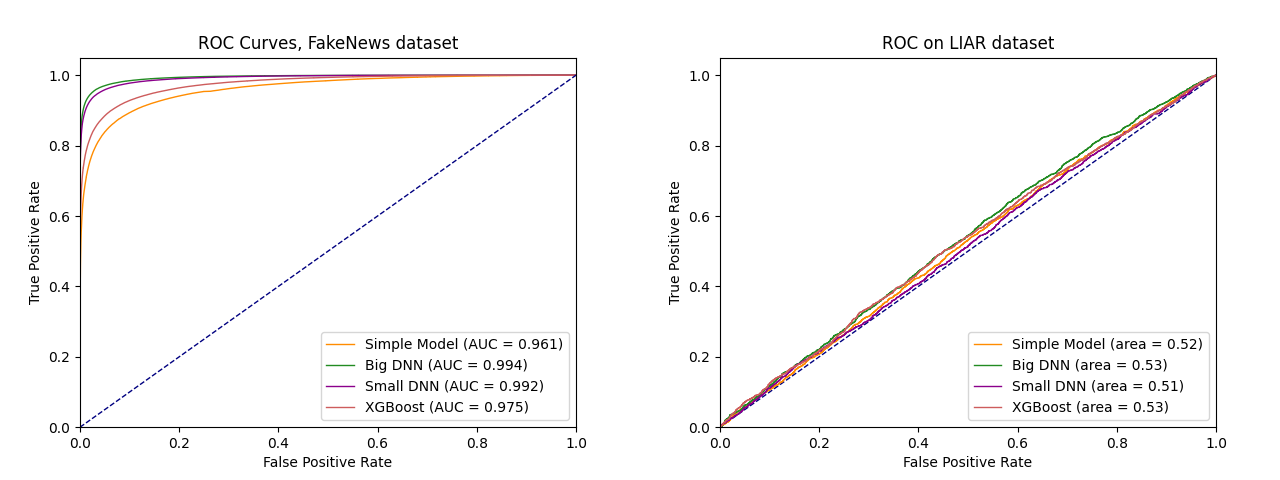
\includegraphics[width=1\textwidth]{figures/ROC_combined}
  \caption{ROC comparison - FakeNewsCorpus and LIAR}
  \label{fig:roc}
\end{figure}


\subsubsection{Inseparability of LIAR on fitted models}
We ran LIAR through the same TF-IDF, SVD and UMAP pipeline to see where they were located in the clusters, we would hope
to see some sort of separation of the various levels of truthiness if we want to have any hope in predicting truthiness
of the LIAR dataset. As seen in the UMAP representation (figure \ref{fig:liarvsfake}), the 6 classes of LIAR are interleaved, which means we will not be able to separate the classes nor make any meaningful inferences on the dataset.

\begin{figure}[htpb]
  \centering
  \includegraphics[width=1\textwidth]{figures/umapLiarVsFake}
  \caption{UMAP - LIAR overlayed on FakeNewsCorpus}
  \label{fig:liarvsfake}
\end{figure}

